\question{}

\begin{lstlisting}
def lit_dipole(nom_De_fichier):
    with open(nom_De_fichier,'r') as f:
        L=f.readlines()
        n=len(L)
        I=[]
        U=[]
        for i in range(1,int(n/2)):
            I.append(float(L[i]))
        for j in range(int(n/2)+1,n):
            U.append(float(L[j]))
        return I,U
\end{lstlisting}

\question{}

\begin{lstlisting}
def tracer_dipole(I,U):
    plt.clf()
    plt.plot(I,U,'r*')
    plt.xlabel('I en (A)')
    plt.ylabel('U en (V)')
    plt.savefig('tp06_durif_q02.png')
\end{lstlisting}



\question{}

Il semble que l'on retrouve bien une relation linéaire entre la tension et l'intensité ce qui est bien conforme à la loi d'ohm.
\begin{center}
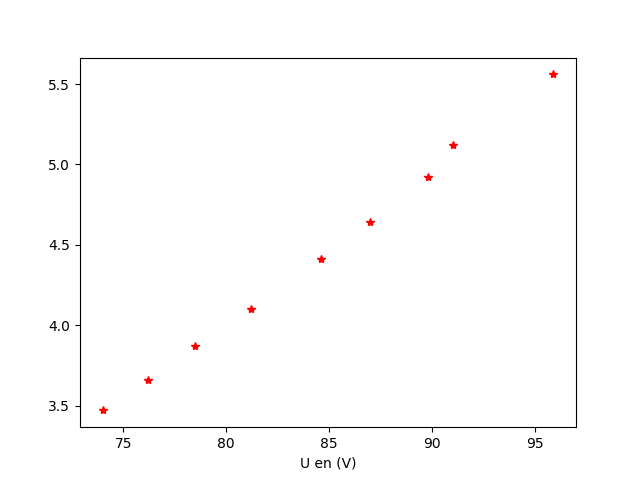
\includegraphics[width=0.5\textwidth]{tp06_durif_q02.png}
\end{center}